\documentclass[tikz,border=2pt]{standalone}
\usepackage{amsmath}
\usepackage{pgfplots}
\pgfplotsset{compat=1.18}
\usetikzlibrary{arrows.meta}
\begin{document}
% Wide table (Belgium 2020/2021, sectors Transport, Buildings, Waste: 22 20 2.1 / 24 21 2.3)
% and its long form with Sector and Emissions columns: 2 rows x 3 sectors = 6 rows.
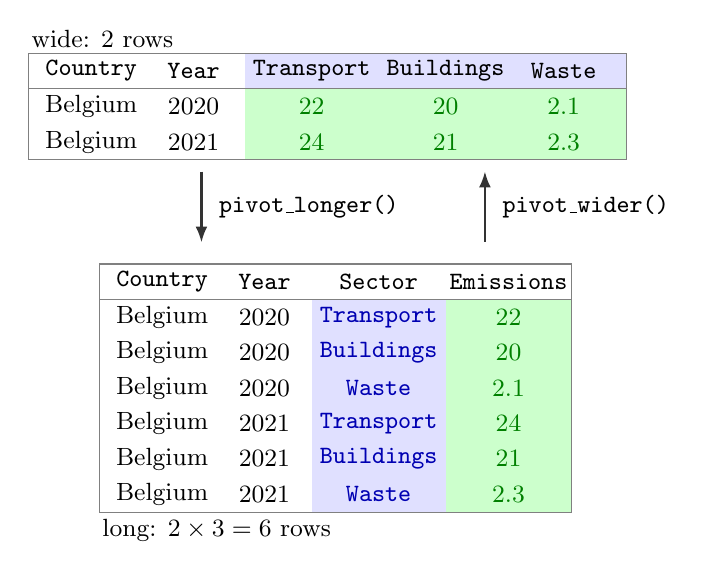
\begin{tikzpicture}[font=\small, >={Latex[length=2mm]},
  hd/.style={font=\small\ttfamily},
  lab/.style={font=\small\ttfamily, anchor=west}]
  \def\h{0.45}
  % ---- wide table, columns at x-centres ----
  \begin{scope}[shift={(0,0)}]
    \fill[blue!12] (2.75,0.5*\h) rectangle (7.6,-0.5*\h);
    \fill[green!20] (2.75,-0.5*\h) rectangle (7.6,-2.5*\h);
    \foreach \x/\t in {0.8/Country,2.1/Year,3.6/Transport,5.3/Buildings,6.8/Waste}
      \node[hd] at (\x,0) {\t};
    \foreach \y/\a/\b/\c [count=\i] in {2020/22/20/2.1,2021/24/21/2.3} {
      \node at (0.8,-\i*\h) {Belgium};
      \node at (2.1,-\i*\h) {\y};
      \node[green!50!black] at (3.6,-\i*\h) {\a};
      \node[green!50!black] at (5.3,-\i*\h) {\b};
      \node[green!50!black] at (6.8,-\i*\h) {\c};
    }
    \draw[gray] (0,-0.5*\h) -- (7.6,-0.5*\h);
    \draw[gray] (0,0.5*\h) rectangle (7.6,-2.5*\h);
    \node[anchor=south west, inner sep=1pt] at (0,0.5*\h+0.03) {wide: 2 rows};
  \end{scope}
  % ---- arrows ----
  \draw[->, thick, gray!40!black] (2.2,-2.5*\h-0.15) -- (2.2,-2.5*\h-1.05);
  \node[lab] at (2.3,-2.5*\h-0.6) {pivot\_longer()};
  \draw[<-, thick, gray!40!black] (5.8,-2.5*\h-0.15) -- (5.8,-2.5*\h-1.05);
  \node[lab] at (5.9,-2.5*\h-0.6) {pivot\_wider()};
  % ---- long table ----
  \begin{scope}[shift={(0.9,-2.5*\h-1.55)}]
    \fill[blue!12] (2.7,-0.5*\h) rectangle (4.4,-6.5*\h);
    \fill[green!20] (4.4,-0.5*\h) rectangle (6.0,-6.5*\h);
    \foreach \x/\t in {0.8/Country,2.1/Year,3.55/Sector,5.2/Emissions}
      \node[hd] at (\x,0) {\t};
    \foreach \y/\s/\v [count=\i] in {2020/Transport/22,2020/Buildings/20,2020/Waste/2.1,2021/Transport/24,2021/Buildings/21,2021/Waste/2.3} {
      \node at (0.8,-\i*\h) {Belgium};
      \node at (2.1,-\i*\h) {\y};
      \node[blue!70!black, font=\small\ttfamily] at (3.55,-\i*\h) {\s};
      \node[green!50!black] at (5.2,-\i*\h) {\v};
    }
    \draw[gray] (0,-0.5*\h) -- (6.0,-0.5*\h);
    \draw[gray] (0,0.5*\h) rectangle (6.0,-6.5*\h);
    \node[anchor=north west, inner sep=1pt] at (0,-6.5*\h-0.05) {long: $2\times3=6$ rows};
  \end{scope}
\end{tikzpicture}
\end{document}
